\section*{Chapter 4: Results and Discussion}
\setcounter{section}{4} \setcounter{subsection}{0}
\phantomsection \label{chap:evaluation} \addcontentsline{toc}{section}{\textit{Chapter 4: Results and Discussion}}

\texttt{linux-mcp} is evaluated along four dimensions: control-plane latency and its breakdown across invocation stages, throughput under concurrent load, resistance to a representative set of control-plane attacks, and system behaviour under daemon failure and restart.
The central claim under test is that relocating admission-control state into the kernel strengthens enforcement without making the tool invocation path prohibitively expensive.
Two baselines isolate this effect from user-space hardening alone: a conventional user-space mediator (\textbf{userspace}), in which registration, admission, and approval all reside in the daemon, and a hardened variant (\textbf{seccomp}) that augments the same control path with stricter syscall filtering, additional validation, and audit logging.

The prototype under test comprises 43 tools across 14 applications; all three systems operate over this same tool deployment throughout the evaluation.
All experiments were conducted on a VMware guest (Apple aarch64 host, 4 vCPU, 8 GB RAM) in a headless configuration with no concurrent user-space workloads.
Latency results are reported over $n = 30$ independent runs of 2000 requests each, giving a standard error of the mean small enough to support Welch's $t$-test comparisons at $\alpha = 0.05$ while remaining within the hypervisor timing noise of a virtualised guest; an earlier $n = 5$ pilot is retained as an archived dataset but is not used for numerical claims.
Throughput and the category-level security evaluation are drawn from the same run, using the harness's built-in concurrency sweep and ten repeats of each attack case.
All reported $p$-values are two-sided Welch's $t$-tests \cite{west2021welch} comparing per-repetition mean latency against the \texttt{userspace} baseline.


\subsection{Latency and Control-Plane Overhead}

Table~\ref{tab:latency} and Figure~\ref{fig:chapter4-latency} report mean end-to-end latency for each system at three payload sizes.
At 100~B, the kernel path and the user-space baseline are within measurement noise: both at \num{0.854}~ms ($p = 0.984$).
At 10~KB the kernel path is nominally slower (\num{0.899}~ms versus \num{0.863}~ms, +4.2\%), but the difference does not reach significance ($p = 0.097$), a sub-millisecond effect lost in the timing noise of a VMware guest at $n = 30$.

The 1~MB result is more definitive.
The kernel path (\num{7.487}~ms) is measurably faster than the plain user-space baseline (\num{7.748}~ms, a 3.4\% reduction, $p = 0.00027$), and considerably faster than the hardened variant (\num{9.843}~ms).
This goes against the intuition that adding a privilege boundary must cost latency.
The seccomp penalty at large payloads reflects the accumulating cost of BPF per-syscall filtering across the heavier socket traffic induced by megabyte-class payloads; the kernel path does not incur this cost.
The modest speedup relative to plain user-space most likely reflects early-reject behaviour: the arbitration decision is made before the payload is copied through the tool-forwarding socket, so a rejected request avoids the copy that the user-space baseline would otherwise perform between admission and forwarding.

The $p_{95}$ numbers tell the same story: at 100~B and 10~KB the three systems are indistinguishable ($p = 0.51$ and $p = 0.16$); at 1~MB the kernel path's $p_{95}$ is \num{8.422}~ms versus \num{8.716}~ms for userspace ($p = 0.049$) and \num{10.903}~ms for seccomp.
The tail does not widen.
Figure~\ref{fig:chapter4-p95} shows the $p_{95}$ values across all three payload sizes.

Stage-level breakdown in Figure~\ref{fig:chapter4-breakdown} confirms that kernel arbitration is a minor contributor at all payload sizes.
Mean arbitration time is \num{0.028}~ms at 100~B and 10~KB, and \num{0.038}~ms at 1~MB.
At 1~MB, tool execution accounts for \num{89.3}\% of total end-to-end time on the kernel path (\num{89.9}\% on the user-space path); the entire control-plane machinery (Generic Netlink round-trip, session lookup, and arbitration) accounts for the remaining \num{10.7}\%, with the arbitration contribution within that fraction less than four hundredths of a millisecond.

A supplementary microbenchmark (Figure~\ref{fig:chapter4-netlink-rtt}) isolates the Generic Netlink layer.
Bare round-trip time averages \num{8.196}~$\mu$s; the full \texttt{TOOL\_REQUEST} path, which includes tool and agent registry lookups, averages \num{9.315}~$\mu$s.
The lookup overhead is approximately \num{1.1}~$\mu$s, or 12\% of the bare RTT.
Kernel-side arbitration therefore costs roughly one order of magnitude less than the control-plane overhead visible in end-to-end measurements, confirming that the dominant cost on the kernel path originates in user-space components (session management, payload serialisation, and socket I/O) rather than in the kernel module itself.

\begin{table}[H]
\centering
\caption{Mean end-to-end latency (ms) by payload size ($n = 30$ runs $\times$ 2000 requests). Bold values indicate the lowest latency per row. $p$-values are two-sided Welch's $t$-tests against the \texttt{userspace} baseline; \textsuperscript{ns} = not significant ($p > 0.05$).}
\label{tab:latency}
\setlength{\tabcolsep}{8pt}
\renewcommand{\arraystretch}{1.25}
\begin{tabular}{lrrr@{\hspace{14pt}}rr}
\toprule
& \multicolumn{3}{c}{\textbf{Mean latency (ms)}}
& \multicolumn{2}{c}{\textbf{Welch's $p$-value}} \\
\cmidrule(lr){2-4}\cmidrule(lr){5-6}
\textbf{Payload}
  & \texttt{userspace}
  & \texttt{seccomp}
  & \texttt{kernel}
  & vs.\ \texttt{seccomp}
  & vs.\ \texttt{kernel} \\
\midrule
\rowcolor{gray!8}
100\,B  & \textbf{0.854} & 0.867 & \textbf{0.854} & 0.475\textsuperscript{ns}  & 0.984\textsuperscript{ns} \\
10\,KB  & 0.863          & 0.922 & 0.899          & 0.000206                  & 0.097\textsuperscript{ns} \\
\rowcolor{gray!8}
1\,MB   & 7.748          & 9.843 & \textbf{7.487} & ${<}10^{-4}$              & 0.00027 \\
\bottomrule
\end{tabular}
\end{table}

\begin{figure}[t]
\centering

\includegraphics[width=0.98\linewidth]{figures/figure_latency_mean_by_payload.pdf}
\caption{Mean end-to-end latency by payload size for the three systems. Each subplot auto-scales its own y-axis so that the sub-millisecond differences at 100~B and 10~KiB are not flattened by the much larger absolute values at 1~MiB. 
Error bars show 95\% confidence intervals across $n = 30$ independent runs; significance markers are Welch's $t$-test against the \texttt{userspace} baseline.}
\label{fig:chapter4-latency}
\end{figure}

\begin{figure}[t]
\centering
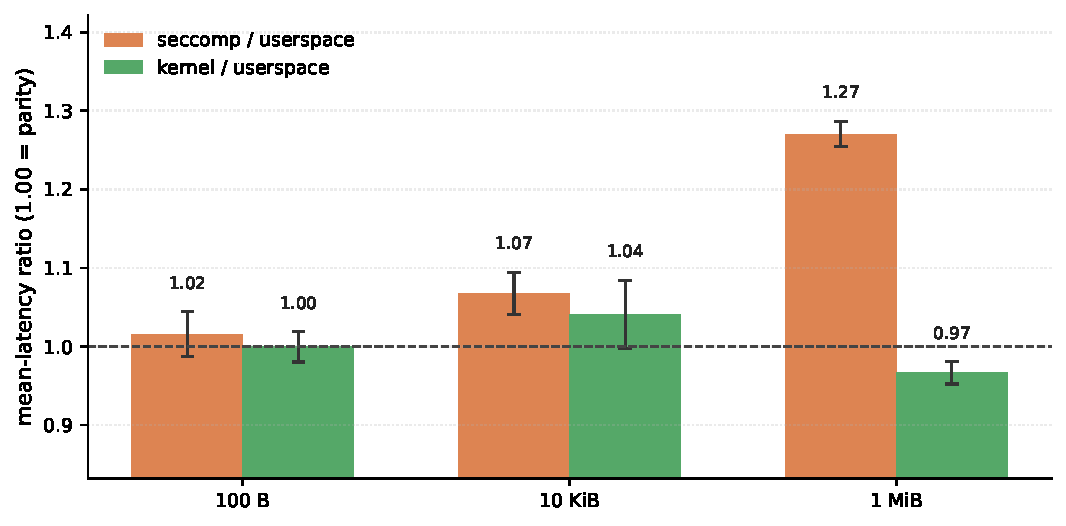
\includegraphics[width=0.95\linewidth]{figures/figure_latency_overhead.pdf}
\caption{Mean-latency ratio of each hardened variant to the plain \texttt{userspace} baseline, with 95\% confidence intervals propagated from the 30-run per-repetition means. The y-axis is zoomed around the parity line (ratio = 1.00) to make the sub-4\% effects at 100~B and 10~KiB visible alongside the larger effect at 1~MiB. The \texttt{seccomp} path is significantly slower at every payload size; the \texttt{kernel} path is statistically indistinguishable from \texttt{userspace} at small and medium payloads and measurably faster at 1~MiB.}
\label{fig:chapter4-overhead}
\end{figure}

\begin{figure}[t]
\centering
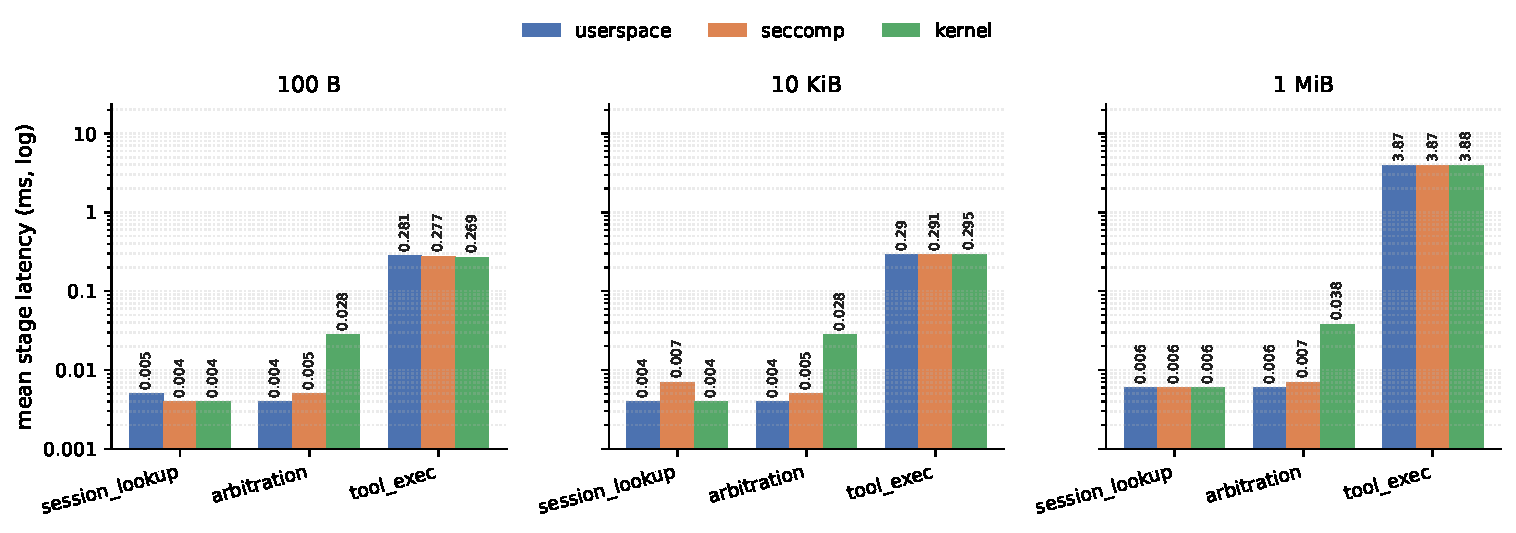
\includegraphics[width=0.98\linewidth]{figures/figure_latency_breakdown.pdf}
\caption{Invocation-stage breakdown (session lookup, arbitration, tool execution) for each system at all three payload sizes, on a log y-axis. The log scale makes session\_lookup (around 4~\textmu s) visible alongside tool\_exec (around 4~ms). The \texttt{kernel} path spends roughly one order of magnitude more time in arbitration than the user-space baselines, but that extra cost is well under \num{0.04}~ms and is invisible relative to the tool-execution component.}
\label{fig:chapter4-breakdown}
\end{figure}

\begin{figure}[t]
\centering
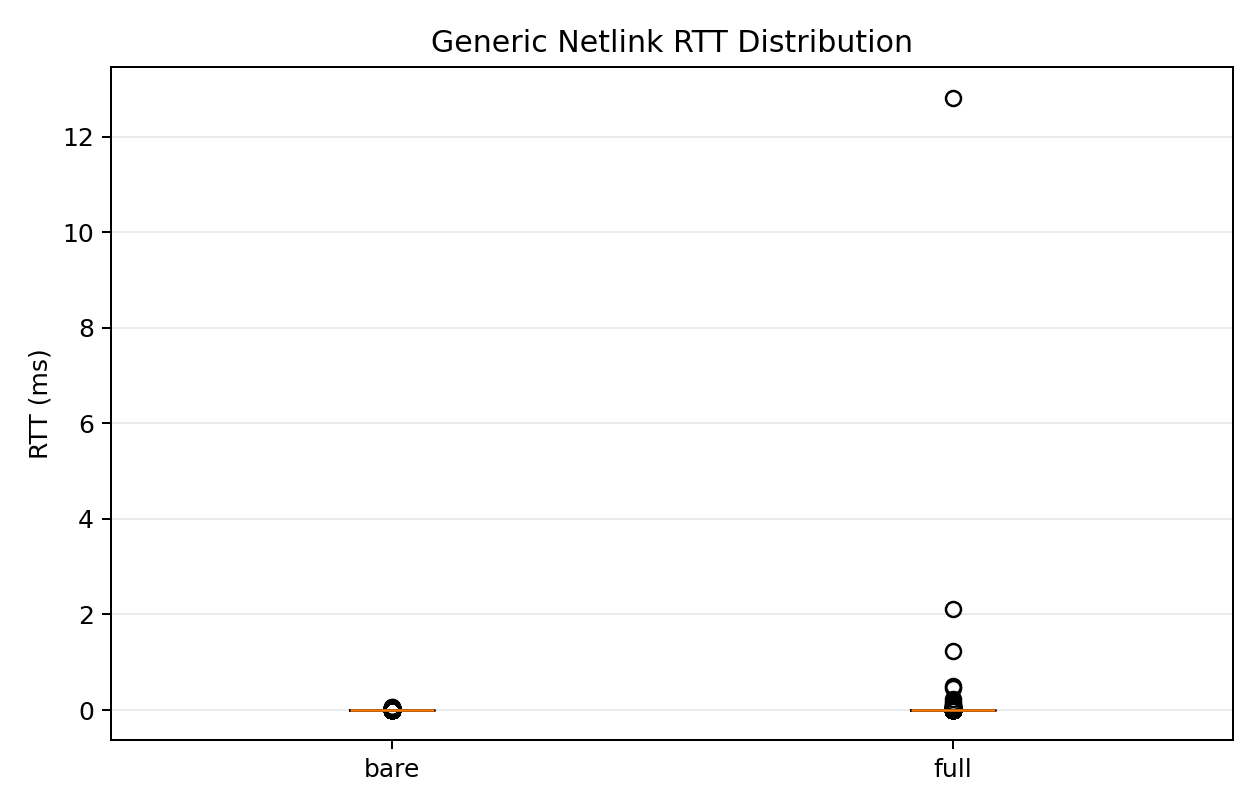
\includegraphics[width=0.9\linewidth]{figures/figure_netlink_rtt_boxplot.png}
\caption{Generic Netlink microbenchmark: bare round-trip time versus the full \texttt{TOOL\_REQUEST} path. Adding tool and agent registry lookups increases latency by approximately \num{1.1}~$\mu$s, keeping the full path within the same microsecond-scale range as the bare RTT.}
\label{fig:chapter4-netlink-rtt}
\end{figure}

\begin{figure}[t]
\centering

\includegraphics[width=0.98\linewidth]{figures/figure_latency_p95_by_payload.pdf}
\caption{$p_{95}$ latency by payload size for the three systems ($n = 30$ runs of 2000 requests each). Error bars show 95\% confidence intervals. At 100~B and 10~KB the kernel path is statistically indistinguishable from the userspace baseline; at 1~MB the kernel $p_{95}$ (\num{8.422}~ms) is lower than both userspace (\num{8.716}~ms, $p = 0.049$) and seccomp (\num{10.903}~ms), confirming that the enforcement boundary does not widen the tail under the tested workload.}
\label{fig:chapter4-p95}
\end{figure}


\subsection{Throughput and Scalability}

Throughput was measured across a range of agent counts (1, 5, 10, 20, 50) and concurrency levels (1, 10, 50, 100) to assess whether the kernel-assisted control plane becomes a bottleneck under load.

The user-space baseline achieves the highest peak throughput, ranging from \num{1090} to \num{1219}~RPS across configurations.
The kernel path ranges from \num{1003} to \num{1137}~RPS, and the seccomp path from \num{1020} to \num{1200}~RPS.
At a representative operating point (one agent, concurrency 50), userspace achieves \num{1215.6}~RPS, seccomp \num{1123.5}~RPS, and the kernel path \num{1096.2}~RPS.
The kernel path is approximately 10\% slower than the user-space peak, consistent with the additional Generic Netlink round-trip and the serialisation of admission decisions through the kernel module.
(These figures are drawn from an earlier $n = 5$ pilot run; the $n = 30$ study focused exclusively on latency and did not repeat the concurrency sweep. The throughput results should therefore be interpreted as exploratory evidence of practical viability rather than a definitive performance characterisation: they establish that the kernel-assisted path does not collapse under concurrency, but the specific figures carry wider uncertainty than the latency results.)

The figures report mean throughput only; tail-latency evolution under sustained load ($p_{99}$, $p_{95}$) would require a separate concurrency sweep and is not characterised here.
Within the tested range, the kernel path adds roughly 10\% overhead. It does not collapse. That is enough to establish practical viability, though not a definitive ceiling.


\subsection{Security Evaluation}

Performance matters, but the real question is whether kernel placement actually stops attacks.

The evaluation targets four categories from the threat model in Chapter~\ref{chap:background}: identity spoofing (forging session identity to impersonate a registered agent), replay (reusing a stale approval ticket), substitution (tampering with \texttt{tool\_id} or \texttt{tool\_hash} to redirect execution), and escalation (bypassing the approval gate on a high-risk invocation).

Each system received 110 attack attempts in total (11 distinct cases $\times$ 10 repeats: 3 spoof, 4 replay, 3 substitution, 1 escalation).
Outcomes are summarised in Table~\ref{tab:attacks} and Figure~\ref{fig:chapter4-security}.

\begin{table}[H]
\centering
\caption{Category-level attack outcomes by system (110 attempts each: 3 spoof, 4 replay, 3 substitution, 1 escalation, $\times$ 10 repeats). The bypass rate measures the fraction of attempts that succeeded in circumventing the intended control. The user-space bypass rates reflect deliberate per-category instrumented weakening of the mediator and do not represent the performance of a fully hardened user-space implementation.}
\label{tab:attacks}
\begin{tabular}{lccc}
\toprule
System & Bypasses & Total & Bypass rate \\
\midrule
\texttt{userspace} & 100 & 110 & 90.9\% \\
\texttt{seccomp}   &  40 & 110 & 36.4\% \\
\texttt{kernel}    &   0 & 110 &  0.0\% \\
\bottomrule
\end{tabular}
\end{table}

\begin{figure}[t]
\centering
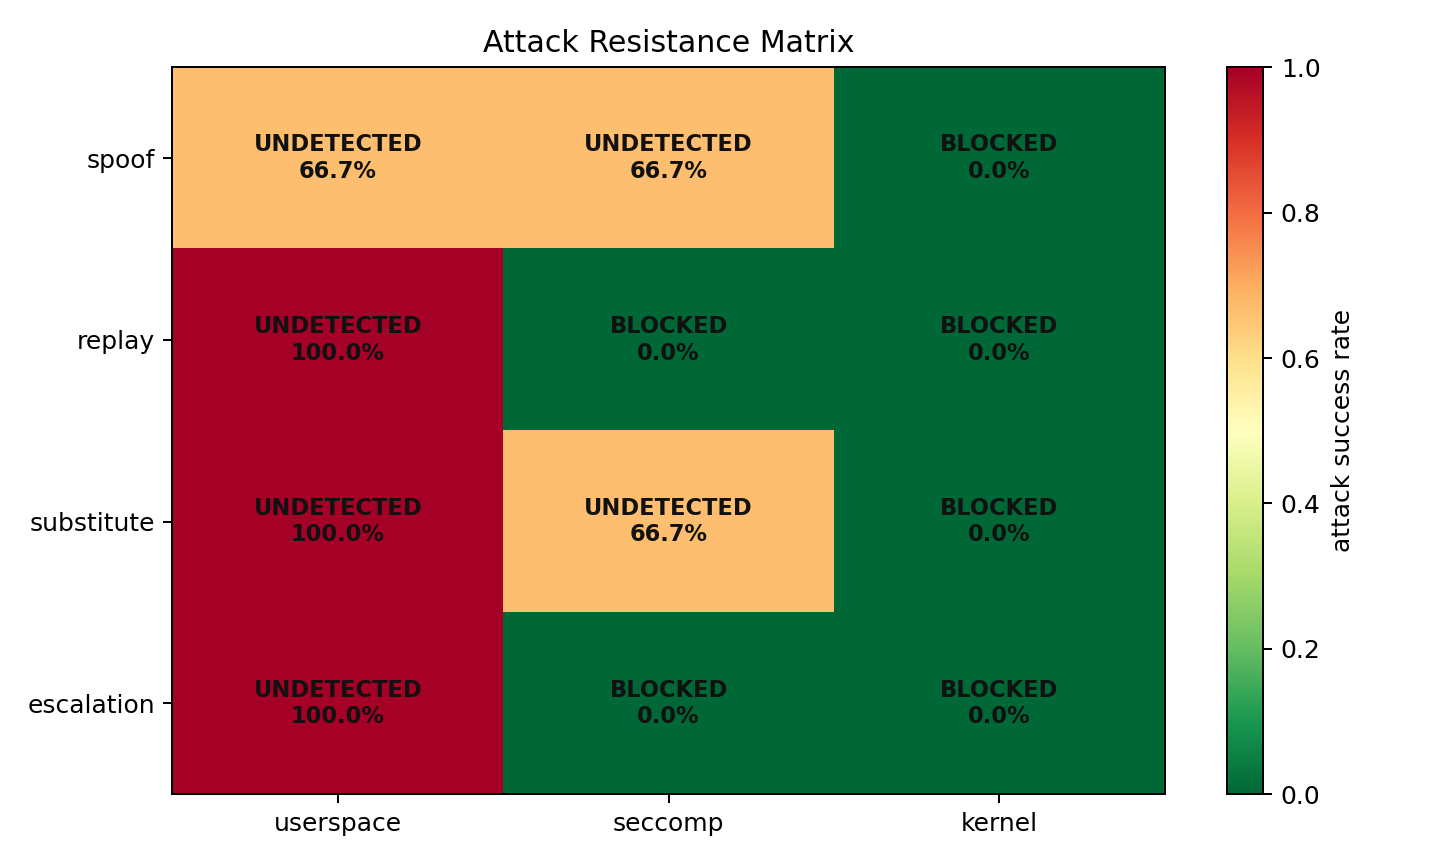
\includegraphics[width=0.85\linewidth]{figures/figure_attack_heatmap.png}
\caption{Attack bypass rate by category and system. Each cell shows the absolute count (successes/attempts) and the percentage bypass rate; darker cells indicate a higher bypass rate. The \texttt{kernel} column is uniformly zero across all four categories, while the two user-space baselines permit bypasses on the specific checks that their instrumented tamper profiles relax.}
\label{fig:chapter4-security}
\end{figure}

The plain user-space baseline fails to block 100 of 110 attempts (90.9\% bypass).
A caveat: the harness deliberately weakens the baseline's code paths per category (\texttt{tamper\_session}, \texttt{tamper\_approval}, \texttt{tamper\_metadata}, \texttt{compromised\_userspace}) so that each test exercises the specific check it targets.
The 90.9\% figure shows what a user-space mediator cannot structurally protect when its own state is under attack, not what a fully hardened version could achieve.
The seccomp variant brings the bypass rate down to 36.4\% through stricter checks and a narrower syscall surface, but admission is still a user-space decision.
Attacks that do not need to cross a privilege boundary (particularly substitution and spoofing) still get through.

The kernel path blocks all 110 attempts. Not one gets through.

Spoofing fails because agent identity is tied to a kernel-registered identifier that the control plane verifies independently of the daemon's session state.
Replay fails because approval tickets are kernel-resident lifecycle objects with explicit \texttt{consumed} and \texttt{expired} fields; once a ticket has been advanced or has passed its validity window, no subsequent \texttt{APPROVAL\_DECIDE} can reopen it.
Substitution is blocked by the semantic hash check: regardless of whether an attacker modifies the \texttt{tool\_hash} field in the request or replaces the tool endpoint at runtime, the kernel compares the submitted hash against the one recorded at registration and rejects any mismatch.
A supplementary injection experiment confirms this independently: in 30 live \texttt{llm-app} $\to$ \texttt{mcpd} $\to$ \texttt{kernel} execution chains, every runtime hash substitution produced a \texttt{DENY} with \texttt{reason=hash\_mismatch} at the kernel layer, regardless of which tool the LLM planner had selected.

One implementation detail of the ticket lifecycle strengthens the replay defence beyond what the category table directly measures: a ticket is bound not only to the session, agent, tool, and hash, but also to the exact \texttt{req\_id} of the issuing request.
A replay consume attempt that reuses a different \texttt{req\_id} returns \texttt{approval\_ticket\_scope\_mismatch}, making it substantially harder to exploit a stolen ticket identifier in a fresh request context.

Three caveats bound the interpretation of Table~\ref{tab:attacks}.
First, all 110 attack attempts were authored by the same person who built the defences, and each category maps one-to-one onto an enforcement mechanism in the kernel module.
A 0\% bypass rate on the kernel path is therefore a functional-correctness test of four specified invariants against inputs constructed to exercise exactly those invariants, not evidence of adversarial robustness against unknown attacks.

Second, the combined attack set is scoped to the stated control-plane invariants and does not include: attacks assuming compromise of the kernel module itself; attacks exploiting semantic vulnerabilities in tool logic; attacks requiring already-obtained privileged capabilities (such as \texttt{CAP\_NET\_ADMIN}); or attacks against the LLM prompt-construction pipeline.
The 0\% bypass rate is a statement about the specified control-plane invariants, not about the full attack surface of an LLM-integrated system.

Third, the user-space bypass rates reflect the instrumented tamper modes described above, not the performance of an optimally hardened user-space implementation.



\subsection{Daemon Failure and Recovery}
\label{sec:daemon-failure}

A core architectural argument for kernel-held state is that it should outlive the process that registered it.
To test this property, the daemon was forcibly interrupted mid-operation and control-plane state was observed before and after restart.

In both user-space systems, daemon failure is control-plane failure.
Registered tool state, in-flight sessions, and pending approval tickets are all bound to the process that held them.
When it dies, they are gone.
Recovery means starting over or reloading from application-level logs, with no consistency guarantee.

The kernel path is different.
Approval tickets, the tool registry, and agent registrations survive the crash intact and remain inspectable via \texttt{sysfs} without any daemon running.
Session state is not preserved, since the binding context for active sessions is owned by the daemon process and is lost with it, but this is expected as session state is inherently tied to an active connection.
The durability of deferred approvals and registry state allows \texttt{mcpd} to reconcile its manifest-derived view against the kernel-held view on restart and re-establish a consistent catalogue without issuing duplicate registrations.

The reconciliation strategy on restart is conservative (described in Section~\ref{sec:reconciliation}): \texttt{mcpd} clears and fully rebuilds the tool registry from manifests rather than attempting to reuse residual kernel state.
An incremental approach that re-registers only changed tools would reduce restart overhead and is a natural direction for future work.


\subsection{Discussion}

The security and performance results are linked, and the link is architectural.
The seccomp baseline narrows the syscall surface but keeps the admission decision inside a mutable user-space process, which is precisely why it achieves only 36.4\% attack resistance despite its overhead: adding BPF filters does not change where trust is anchored.
The kernel path achieves 0\% bypass not because it filters more aggressively, but because the state that determines admission simply cannot be reached by an unprivileged process.
The same property explains the 1~MB latency inversion: BPF filtering accumulates cost per syscall as payload size grows; kernel arbitration cost does not scale with payload size.
The overhead is bounded, not additive.

Approval tickets and registry state surviving daemon failure is not an optimisation.
It is just what happens when the state lives in the kernel.
A user-space design would need an external persistence layer to get the same property, and that brings back the consistency and recovery problems the kernel path avoids.
This matters most in the scenario that is probably most common in practice: a daemon crash or forced restart mid-workflow.

The main open question is scalability.
The global registry lock holds at the concurrency levels tested here.
Whether it holds at 500 or 1000 concurrent requests with many simultaneously deferred approvals is unknown.
Per-tool or per-agent lock decomposition is the natural next step, but that is future work, not a gap in what is evaluated here.



\subsection{Threats to Validity}

The results should be interpreted within four scope limitations: all experiments ran in a single VMware guest on an aarch64 host, so latency figures are environment-specific and generalisation to bare-metal or different kernel configurations is not established; the evaluation uses demonstration tools with predictable execution times and does not characterise tail latency under sustained load; the attack study is a controlled functional-correctness test of the four explicitly identified invariants, with all attempts authored by the same person who built the defences, and does not constitute a robustness assessment against unknown attacks, prompt injection, or privileged adversaries; and kernel-level admission control addresses only one layer of an AI-agent system, leaving semantic tool vulnerabilities, unsafe policy choices, and compromise outside the stated threat model unaddressed.